\section{}
A tube acts as a water siphon. Determine the speed of jet and the
minimum pressure of water in the bend (at the point A).

\begin{figure}[h]
    \centering
    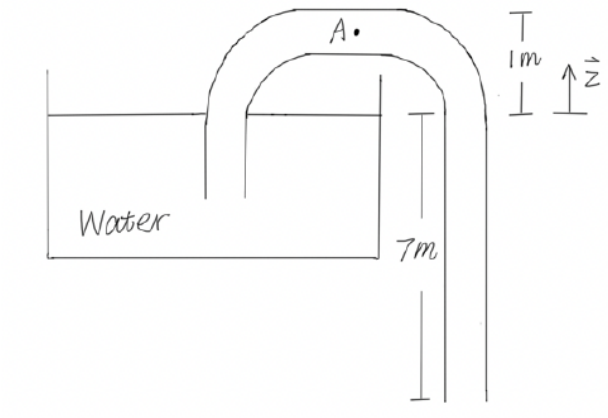
\includegraphics[width=0.5\linewidth]{Questions/Figures/Q1ProblemDiagram.png}
    \caption{Tube with water siphon}
    \label{fig:Q1ProblemDiagram}
\end{figure}

\textbf{Solution} \\
Assumptions:
\begin{itemize}
    \item Steady flow
    \item Incompressible flow
    \item Negligible viscous effects
    \item Negligible diameter change
    \item Reservoir is large enough to be considered infinite
\end{itemize}

By the Bernoulli equation, the speed of jet is given by:
\begin{gather*}
    \underbrace{\cancel{\frac{P_1}{\rho} - \frac{P_2}{\rho}}}_{\text{Both exposed to atm}} + \frac{v_2^2}{2} - \underbrace{\cancel{\frac{v_1^2}{2}}}_{\text{large reservoir}} + g(z_2 - z_1) = 0 \\
    \frac{v_2^2}{2} + g(z_2 - z_1) = 0 
\end{gather*}

Which results in
\begin{align*}
    v_2 &= \sqrt{2g(z_1 - z_2)} \\
    &= \sqrt{2(9.81)(7)} \\
    &= \boxed{\qty{11.7}{\meter\per\second}}
\end{align*}

In the pipe, by the assumptions, the velocity is constant. Therefore taking the Bernoulli equation between the pipe exit and the bend, 
\begin{gather*}
    \frac{P_A}{\rho} - \frac{P_2}{\rho} + \cancel{\frac{v_A^2}{2} - \frac{v_2^2}{2}} + g(z_A - z_2) = 0 \\
    \frac{P_A}{\rho} - \frac{P_2}{\rho} + g(z_A - z_2) = 0 \\
\end{gather*}

Rearranging for $P_A$,
\begin{align*}
    P_A &= \rho g(z_2 - z_A) + P_2 \\
    &= (1000)(9.81)(-7 - 1) + 101325 \\
    &= \boxed{\qty{22.84}{\kilo\pascal}}
\end{align*}